\documentclass[12pt,a4paper]{article}
\usepackage[margin=1in, top=1in, bottom=1in]{geometry}
\usepackage{amsmath,etoolbox}
\usepackage{lipsum}
\usepackage{fancyhdr}
\usepackage{graphicx}
\graphicspath{ {images/} }
\usepackage{libertine}  % For times new roman equivalent linux
\usepackage[T1]{fontenc}

\renewcommand{\contentsname}{Table of Contents}  % Contents will be called Table of Commands

\newcommand{\projecttitle}{Ecobot}  % Title of the project

\newcommand{\teamleaderfirst}{Lakshay}
\newcommand{\teamleaderlast}{Garg}
\newcommand{\teamleaderemail}{
  \makeatletter
  lakshayg@iitk.ac.in
  \makeatother
}

\newcommand{\othermemberfirstandlast}{
  \makeatletter
  Abhibhav Garg, & abhibhav@iitk.ac.in\\
  Pranjal Giri, & prgiri@iitk.ac.in\\
  Shubham P. Jain, & spjain@iitk.ac.in\\
  Yash Srivastav, & yashsriv@iitk.ac.in
  \makeatother
}
\newcommand{\othermemberfirst}{
  Abhibhav\\
  Pranjal\\
  SP\\
  Yash
}

% First title page
\newcommand{\titleone}{
  \projecttitle{} \\
  Robocon 2016 \\
  Prof. B. Dasgupta \\
  \begin{tabular}{r l}
    \teamleaderfirst{} \teamleaderlast{}, & \teamleaderemail{} \\
    \othermemberfirstandlast{} \\
  \end{tabular}\\
  \today
}
% Second title page
\newcommand{\titletwo}{
  \projecttitle{} \\
  Robocon 2016 \\
  Prof. B. Dasgupta \\
  \teamleaderfirst{}\\
  \othermemberfirst{} \\
  \today
}

\pagestyle{fancy}
\fancyhf{}
\chead{\teamleaderfirst, et al.}
\rfoot{\thepage}
\lfoot{\today}

% Beginning document
\begin{document}

  % Roman Page numbering and centered text for title pages
  \pagenumbering{roman}
  \centering

  \addcontentsline{toc}{section}{\protect\numberline{}Title Pages}% Add title to ToC

  % Page 1
  \thispagestyle{plain}
  \titleone{}
  \clearpage
  % Page 2
  \thispagestyle{plain}
  \titletwo{}
  \newpage

  % Left aligned text throughout
  \raggedright
  \thispagestyle{plain}

  % Generate ToC and add ToC to ToC
  {
    \makeatletter
    \let\@oldstarttoc\@starttoc
    \renewcommand{\@starttoc}{%
      \addcontentsline{toc}{section}{\protect\numberline{}\contentsname}% Add ToC to ToC
      \@oldstarttoc
    }
    \tableofcontents
    \makeatother
  }
  \newpage


  % Page Numbering Settings begin

  \numberwithin{page}{subsection}% Number page by subsection

  % Make sure that page starts from 1 with every \subsection
  \makeatletter
  \patchcmd{\@sect}% <cmd>
    {\protected@edef}% <search>
      {\def\arg{#1}\def\arg@{subsection}%
      \ifx\arg\arg@\stepcounter{page}\fi%
      \protected@edef}% <replace>
  {}{}% <success><failure>
  \makeatother

  \renewcommand{\thepage}{\thesubsection.\arabic{page}}% Page numbering style

  % Page Numbering Settings end

  \section{Project Management Plan}
    \subsection{Overview}
      Robocon 2016 organised by ABU Robocon with the theme \textbf{Clean Energy Recharging the World}.
      The game of ABU Robocon 2016 is designed in order to create the 
      awareness of efficient energy consumption and clean and renewable 
      energy utilization. Each team has to build two robots; Eco Robot 
      and Hybrid Robot. Eco Robot does not have an actuator to drive. 
      It receives the driving energy from Hybrid Robot. Eco Robot has 
      to use only one steering actuator to control its direction, to 
      track the path containing Slopes and Hills, River, and Down Hill. 
      Besides providing driving energy to Eco Robot, Hybrid Robot has to 
      take Wind Turbine Propeller from Eco Robot and climb up Wind Turbine 
      Pole in order to assemble Wind Turbine.\vspace{2mm}\\
      Contest Ideas:
      \begin{itemize}
        \item The team utilizes limited resources to design the robot's mechanisms 
              and strategies to accomplish the assigned tasks
        \item The game is challenging for the contestants
        \item The game is easy to understand and entertains the spectators
        \item The automatic control technique is emphasized in this game
        \item The winner of each game is not predictable till the end
      \end{itemize}
    \clearpage
    \subsection{Scope and Objectives}
      This team was responsible for programming the ecobot and ensuring that 
      it took the game arena perfectly.\\
      \begin{itemize}
        \item Achieve Line Following on the ecobot such that it can cover the game arena reliably
      \end{itemize}
      \begin{figure}[h]
        \centering
        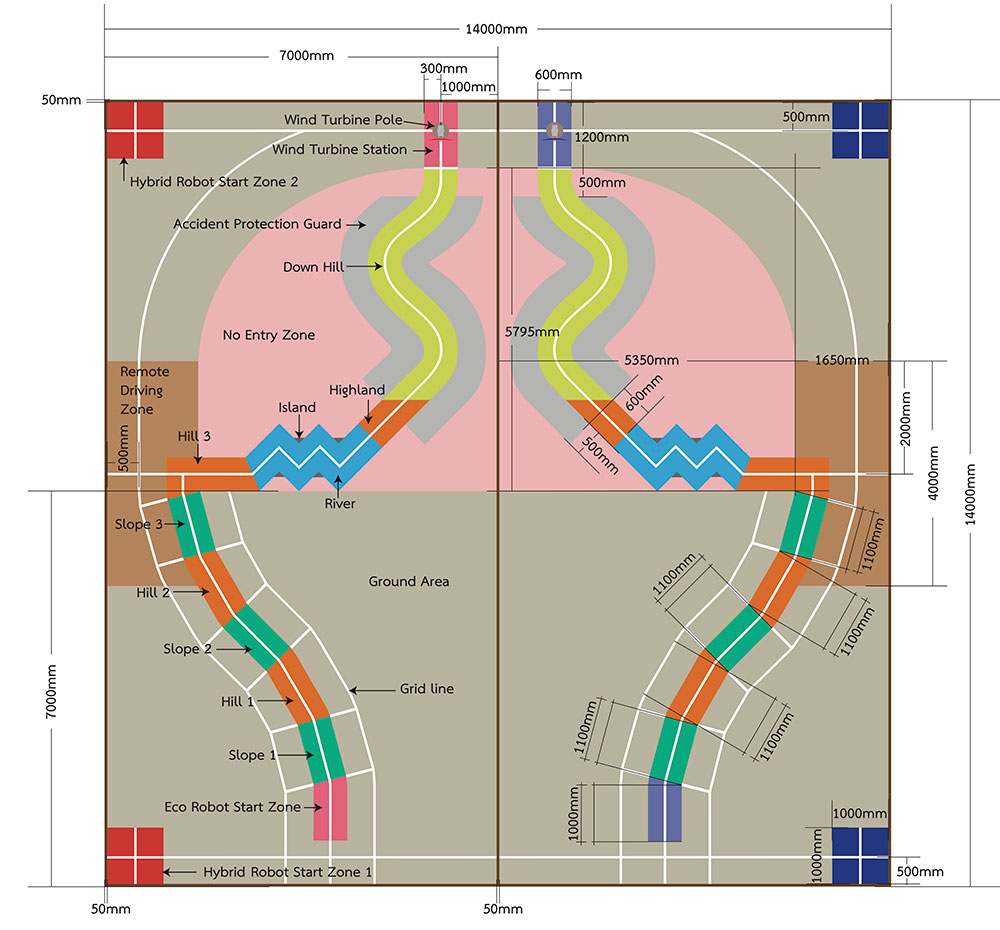
\includegraphics[width=\textwidth]{gamefield}
        \caption{The Game Field}
      \end{figure}
    \clearpage
    \subsection{Assignment of Roles and Responsibilities}
      Roles :\\
      \begin{itemize}
        \item Lakshay Garg - Team Leader, Programmer, Tester
        \item Abhibhav Garg - Tester, Programmer
        \item Pranjal Giri - Programmer
        \item Shubham Jain - Tester, Backup Specialist
        \item Yash Srivastav - Programmer, Tester
      \end{itemize}
      Responsibilities :\\
      \begin{itemize}
        \item Programmer - Program the ecobot to complete the game arena in any way possible
        \item Tester - Test the ecobot on the arena to find flaws and errors in the algorithm used
        \item Backup Specialist - Delete the code
      \end{itemize}
    \clearpage
    \subsection{Project Schedule}
      \lipsum[1]
    \clearpage

  \section{Requirements Specifications}
    \subsection{}
      \lipsum[15-20]
    \clearpage

  \section{Analysis}
    \subsection{Introduction}
      Initial atempts were to achieve line following via a line sensor  
      and then cover the river region using a combination of data from  
      the line sensor and ultrasonics mounted on the sides to cover  
      the rest of the arena \par
      However the line sensors were found unreliable for varying lighting  
      conditions and it was ultimately decided that we should use Image  
      Processing to achieve line following as well as color detection for  
      optimized line following based on which portion of the arena the ecobot was in
    \clearpage
    \subsection{Equipment Used}
      \begin{itemize}
        \item
          \begin{figure}[h!]
            \centering
            \caption{Odroid U3}
            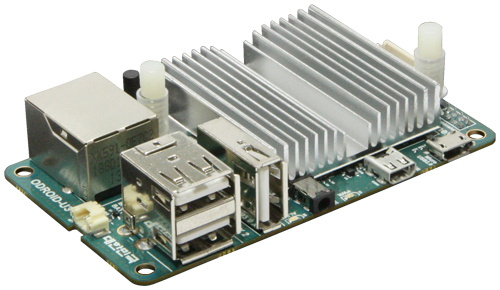
\includegraphics[width=0.25\textwidth]{odroid}
          \end{figure}
        \item
          \begin{figure}[h!]
            \centering
            \caption{I/O Shield for the odroid}
            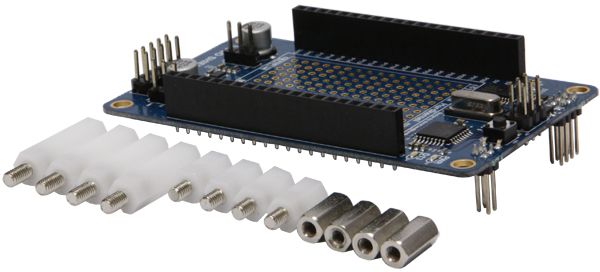
\includegraphics[width=0.25\textwidth]{ioshield}
          \end{figure}
        \item
          \begin{figure}[h!]
            \centering
            \caption{Web Camera(Creative VF-0060)}
            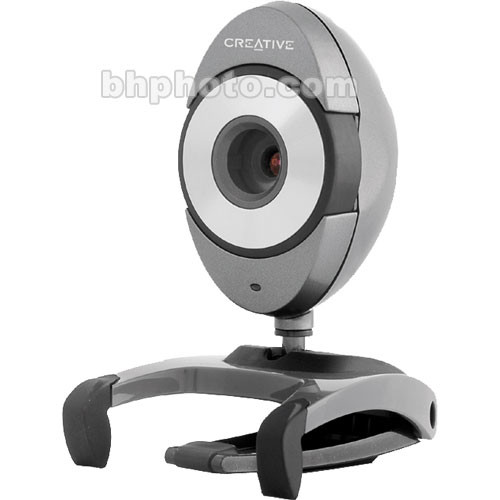
\includegraphics[width=0.25\textwidth]{webcam}
          \end{figure}
        \item
          \begin{figure}[h!]
            \centering
            \caption{Servo Motor}
            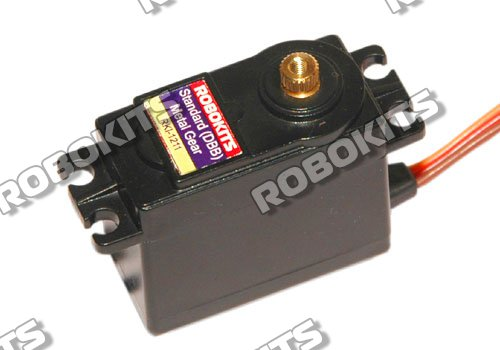
\includegraphics[width=0.25\textwidth]{servo}
          \end{figure}
      \end{itemize}
      \clearpage

  \section{Design}
    \subsection{}
      \lipsum[15-20]
    \clearpage

  \section{Implementation}
    \subsection{}
      \lipsum[15-20]
    \clearpage

  \section{Test Documentation}
    \subsection{}
      \lipsum[15-20]
    \clearpage

  \section{Appendices}
    \renewcommand{\thepage}{A.\arabic{page}}% Page numbering style
    \subsection{Glossary}
      \lipsum[1-5]
    \clearpage
    \renewcommand{\thepage}{B.\arabic{page}}% Page numbering style
    \subsection{Source Code}
      \lipsum[1-5]
    \clearpage
    \renewcommand{\thepage}{C.\arabic{page}}% Page numbering style
    \subsection{Version Index}
      \lipsum[1-5]
    \clearpage
    \renewcommand{\thepage}{D.\arabic{page}}% Page numbering style
    \subsection{References}
      \lipsum[1-15]
    \clearpage

\end{document}
